Betrachten Sie folgendes Klassendiagramm, welches leider ungültig ist:



\begin{centering}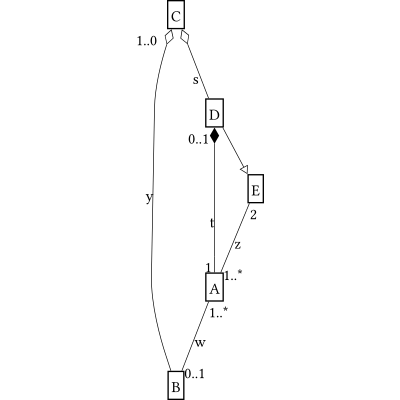
\includegraphics[min width=0.4\textwidth=0.6\textwidth,min height=0.4\textwidth=0.6\textwidth,keepaspectratio,max width=0.9\textwidth,max height=0.9\textwidth]{55/cd37ac6ad6ed2c227b4b30e91fae819c9c1cdefc064aad85ece210411452eaf1b801af83b04c596701db35357ce8aed00a3a92e08161.pdf}\end{centering}



Welche der folgenden Änderungen würden jeweils das Klassendiagramm reparieren?

\begin{enumerate}\item[ 1 ]{ergänze eine Beziehung, die C eine Komposition aus Es macht, wobei C genau einmal und E genau zweimal beteiligt ist,}
\item[ 2 ]{ersetze die Vererbung, bei der D von E erbt, durch eine Vererbung, bei der E von D erbt}
\item[ 3 ]{ersetze Aggregation y durch eine Beziehung, die C eine Komposition aus Bs macht, wobei C genau einmal und B mit der Standardmultiplizität beteiligt ist}
\item[ 4 ]{ersetze Aggregation y durch eine Beziehung, die C eine Komposition aus Bs macht, wobei C 0..1-mal und B mit der Standardmultiplizität beteiligt ist}
\end{enumerate}Bitte geben Sie Ihre Antwort als Liste aller Zahlen an, deren Änderungen jeweils in einem gültigen Klassendiagramm resultieren.

Antworten Sie durch Angabe einer durch Komma separierten Liste aller zutreffenden Optionen. Zum Beispiel \begin{verbatim}[1, 2]\end{verbatim} als Angabe würde bedeuten, dass die Optionen 1 und 2 jeweils das gegebene Klassendiagramm reparieren.

Bitte beachten Sie: Klassen werden hier vereinfacht dargestellt. 
 Das heißt, sie bestehen aus einer einfachen Box, die nur den Klassennamen enthält, aber keine Abschnitte für Attribute oder Methoden. 
 Trotzdem sollten Sie diese vereinfachten Klassendarstellungen als valide Klassen ansehen.

Bitte beachten Sie: Beim Bewegen über oder Klicken auf Kanten / Knoten bzw. ihre Beschriftungen werden die jeweils zusammengehörenden Komponenten hervorgehoben.

